\begin{tikzpicture}
    
    \tikzstyle{lien} = [->, >=latex]
    \tikzstyle{basic_text}=[text width=2cm, text badly centered]
    \tikzstyle{basic_node}=[draw = black,rounded corners=4pt, basic_text]
    \tikzstyle{wrapper}=[basic_node, inner sep=3pt]
    \tikzstyle{hidden}=[draw=black!0,color=black!0]
    \tikzstyle{faded}=[draw=black!20, color=black!20]

    
        \node [basic_node, text width=7cm, align=left] (AS)  {
            
            \scalebox{0.9}{
            \parbox{\textwidth}{
                \textbf{Arbre de syntaxe}
                    
\tikzstyle{feuille}=[ draw, rectangle, inner sep = 0.12cm]
\tikzstyle{noeud}=[ draw, rectangle,rounded corners, minimum width= 0.64cm, line width = 1pt]
\begin{tikzpicture}[
        baseline=(base), 
        level/.style={sibling distance = 1.6cm/#1, level distance = 1cm},
        every node/.style={scale=0.6, font=\footnotesize}
    ]
    
    \node[ noeud] {Programme}
    child { 
        node[noeud] (base) {ProgramMC}
    }
    child {
        node[noeud] {NomProg}
        child {node[feuille] {"hello"}}
    }
    child [ level distance=2cm]{ 
        node [ noeud] {Print}
        child [sibling distance= 1cm] {
            node [noeud] {PrintMC}
        }
        child [sibling distance= 1cm]{
            node [noeud] {Asterisque}
        }
        child [sibling distance= 1cm]{
            node [noeud] {Virgule}
        }
        child [sibling distance= 1cm]{
            node [noeud] {Chaine}
            child { 
                node [feuille] {"Hello World"}
            }
        }
        child [sibling distance= 1cm] {
            node [noeud] {Paramliste}
            child { 
                node [feuille] {$\varepsilon$}
            }
        }
    }
    child { 
        node[ noeud] {EndProgramMC}
    }
    child {
        node[noeud] {NomProg}
        child {node[feuille] {"hello"}}
    };

\end{tikzpicture}}
            }

        };


    \begin{scope}[shift={(6,0)}]
        \node [basic_node, text width=4cm, align=left] (AST){
            \scalebox{0.8}{
                \begin{minipage}{\textwidth}
                    \textbf{Arbre de syntaxe \\abstraite}

                    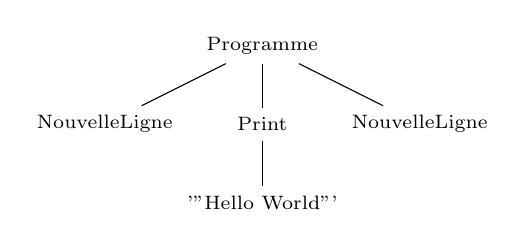
\begin{tikzpicture}
    \node[font=\scriptsize] (0) at (0, 0) {Programme};
    \node[font=\scriptsize] (1) at (-2, -1) {NouvelleLigne};
    \node[font=\scriptsize] (2) at (0, -1) {Print};
    \node[font=\scriptsize] (3) at (0, -2) {'"Hello World"'};
    \node[font=\scriptsize] (4) at (2, -1) {NouvelleLigne};
    
    \draw (0) -- (1);
    \draw (0) -- (2);
    \draw (2) -- (3);
    \draw (0) -- (4);
\end{tikzpicture}
                \end{minipage}

            }
        };
    
    \end{scope};
    \draw [lien] (AS.north east) to[out=45, in=135]  node[midway, above] {\textbf{Conversion en arbre de syntaxe abstraite}}  (AST.north) ; 

\end{tikzpicture}